

\section{Class-Conditional Sampling} %0.5-1
\section{Semantic Synthesis Sampling} %1-2
%%%%%%%%%%%%%%%%%%%%%%%%%%%%%%%%%%%%%%%%%%%%%%%%%%%%%%%%%%%%%%%%%%%%%%%%%%%%%%%%%%%%%%%%%%
\section{Improvements and Adaptations}
As initial experiments before testing semantic image synthesis on a large scale, we test the impact of two improvements/adaptations we made to the original score model architecture \cite{score_3}.
\subsection{Mixed precision learning} %0.5-1
vRAM usage and training speed are key aspects in training deep neural network. Complex models might consist of several million up to billion parameters to optimize. This requires an immense amount of computing power but at least equally important, vRAM. vRAM – video random access memory – is the memory that a GPU has available during operation. Modern high end consumer graphic cards typically have around $10GB$ of vRam. The crux of the matter is that reaching more than $10GB$ when training a moderately complex model is really easy and when training such complex models as NCSNs, the vRAM demand can increase beyond $100GB$ making training deep neural networks a very cost intensive business. Also when training complex models one can expect to need one week or more of training time making testing and finetuning of models very exhausting.

To mitigate these problems the concept of \textit{Mixed Precision Learning} \cite{mixed_prec} was developed, decreasing both vRAM usage and training time with simultaneous retention of training quality, i.e. training loss. Normally each parameter of a network is stored as a float with $32bits$ of precision. Considering a network with $\sim250M$ parameters this would be equivalent to $\sim1GB$. What sounds not so much at first quickly becomes unmanageable when thinking of the series of matrix arithmetic's the parameters undergo and each calculation storing extra data such as gradients. 

The idea of mixed precision learning is to use floats with a $16bit$ precision wherever possible. In order to not loose model accuracy two concepts are applied. First, there is always a $32bit$ master copy of the model weights. For the forward pass this master copy is converted to $16bit$ where the complex gradient calculations happen. In the backward pass these $16bit$ gradients are converted back to $32bit$ where they are then used by the optimizer to update the master weights. But this improvement during gradient calculation comes with the flaw of loosing some gradients as every number $<2^{-24}$ is equal to $0$ for $16bit$ precision but in most models there is at least some relevant gradient information in the range $[2^{-27},2^{-24})$. To mitigate this effect the concept of loss scaling was proposed. Loss scaling multiplies the $32bit$ loss after the forward pass by a scale factor to move them in the $16bit$ range in which the gradients are then computed in the backward pass. Thereafter the scaled $16bit$ gradients are converted to scaled $32bit$ gradients and then divided by the same scale factor as before. Finally these scaled gradients are used by the optimizer to update the master weights. The full concept can be seen in \hyperref[fig:3.2]{Fig. 3.2}.
%
\begin{figure}[] \label{fig:3.2}
    \centering
    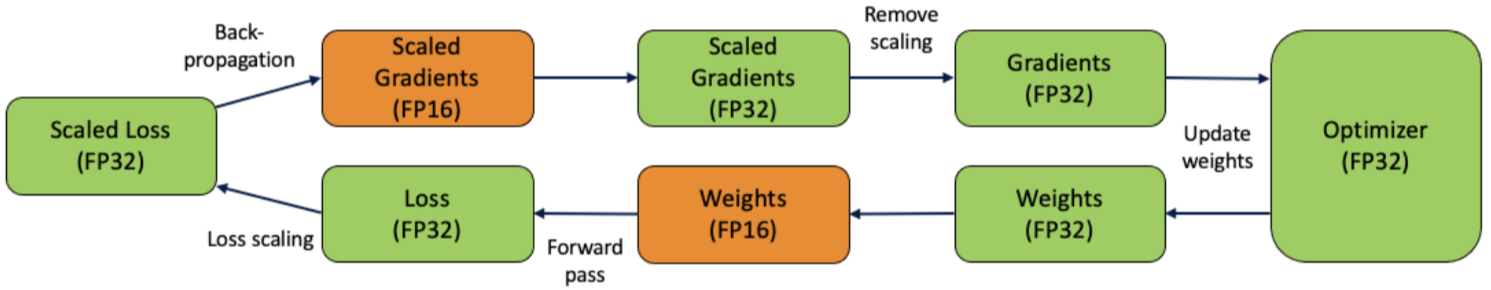
\includegraphics[width=.9\textwidth]{Chapters/figures/mixed_prec.PNG}
    \caption[Short-form caption]{Concept of Mixed Precision}
\end{figure}
%

As the mixed precision technique was not used in the original SGM paper \cite{score_3} it was now implemented using the off the shelf pyTorch tools for mixed precision to check how much this technique improves vRAM usage and training time for the NCSN. To do so the NCSN was trained on the Cityscapes dataset on two different GPUs with the same model settings. For each GPU $2\times100$ epochs were passed, once with mixed precision on and once with mixed precision off. The first GPU was a \textit{Nvidia GeForce RTX 2080 Ti} with $11GB$ of vRAM and the second GPU was a \textit{Nvidia A100} with $40GB$ of vRAM. For both GPUs we used the maximum possible batch size for non mixed precision training which is $1$ for the RTX 2080 Ti and $5$ for the A100. The effects of mixed precision training on vRAM usage and training time can be seen in \hyperref[tab:3.1]{Tab. 3.1} resp. \hyperref[tab:3.1]{Tab. 3.2}. For the vRAM usage the total vRAM needed is shown and for the training time the average training time for one epoch is shown.
%
\begin{table}[] \label{tab:3.1}
        \centering
    \begin{tabular}{c|c|c}
        GPU type        & Mixed precision \textbf{Off}    & Mixed precision \textbf{On} \\
        \hline
        RTX 2080 Ti     &  7791MB               & 7367MB\\
        A100            &  39039MB              & 29481MB
    \end{tabular}
    \caption{vRAM usage w/ and w/o mixed precision}
\end{table}
\begin{table}[b] \label{tab:3.2}
        \centering
    \begin{tabular}{c|c|c}
        GPU type        & Mixed precision \textbf{Off}    & Mixed precision \textbf{On} \\
        \hline
        RTX 2080 Ti     &  1494s                & 1206s    \\
        A100            &  965s                 & 987s
    \end{tabular}
    \caption{Training time per epoch w/ and w/o mixed precision}
\end{table}

For the A100 serious improvements on vRAM usage can be observed. For the RTX 2080 Ti there are only little improvements for vRAM usage but good improvements on training time. In general mixed precision is expected to perform way better on the new Ampere GPU
architecture (A100) than on the older Turing GPU architecture (RTX 2080 Ti). To ensure that the training quality does not suffer from the use of mixed precision the loss curves for all test setups are compared in \hyperref[fig:3.3]{Fig. 3.3}. The higher fluctuations for the RTX 2080 Ti are due to the fact that the batch size is smaller, therefore leading to major loss differences in a batch-to-batch comparison. In general it can be seen that mixed precision has no notable effect on training loss. Also a qualitative comparison of generated samples shows no difference perceptible by a human. We therefore conclude that – at least for non FID record breaking attempts – mixed precision should be used and we do so for all upcoming experiments.
%
\begin{figure} \label{fig:3.3}
    \centering
    \begin{subfigure}[b]{0.49\textwidth}
        \centering
         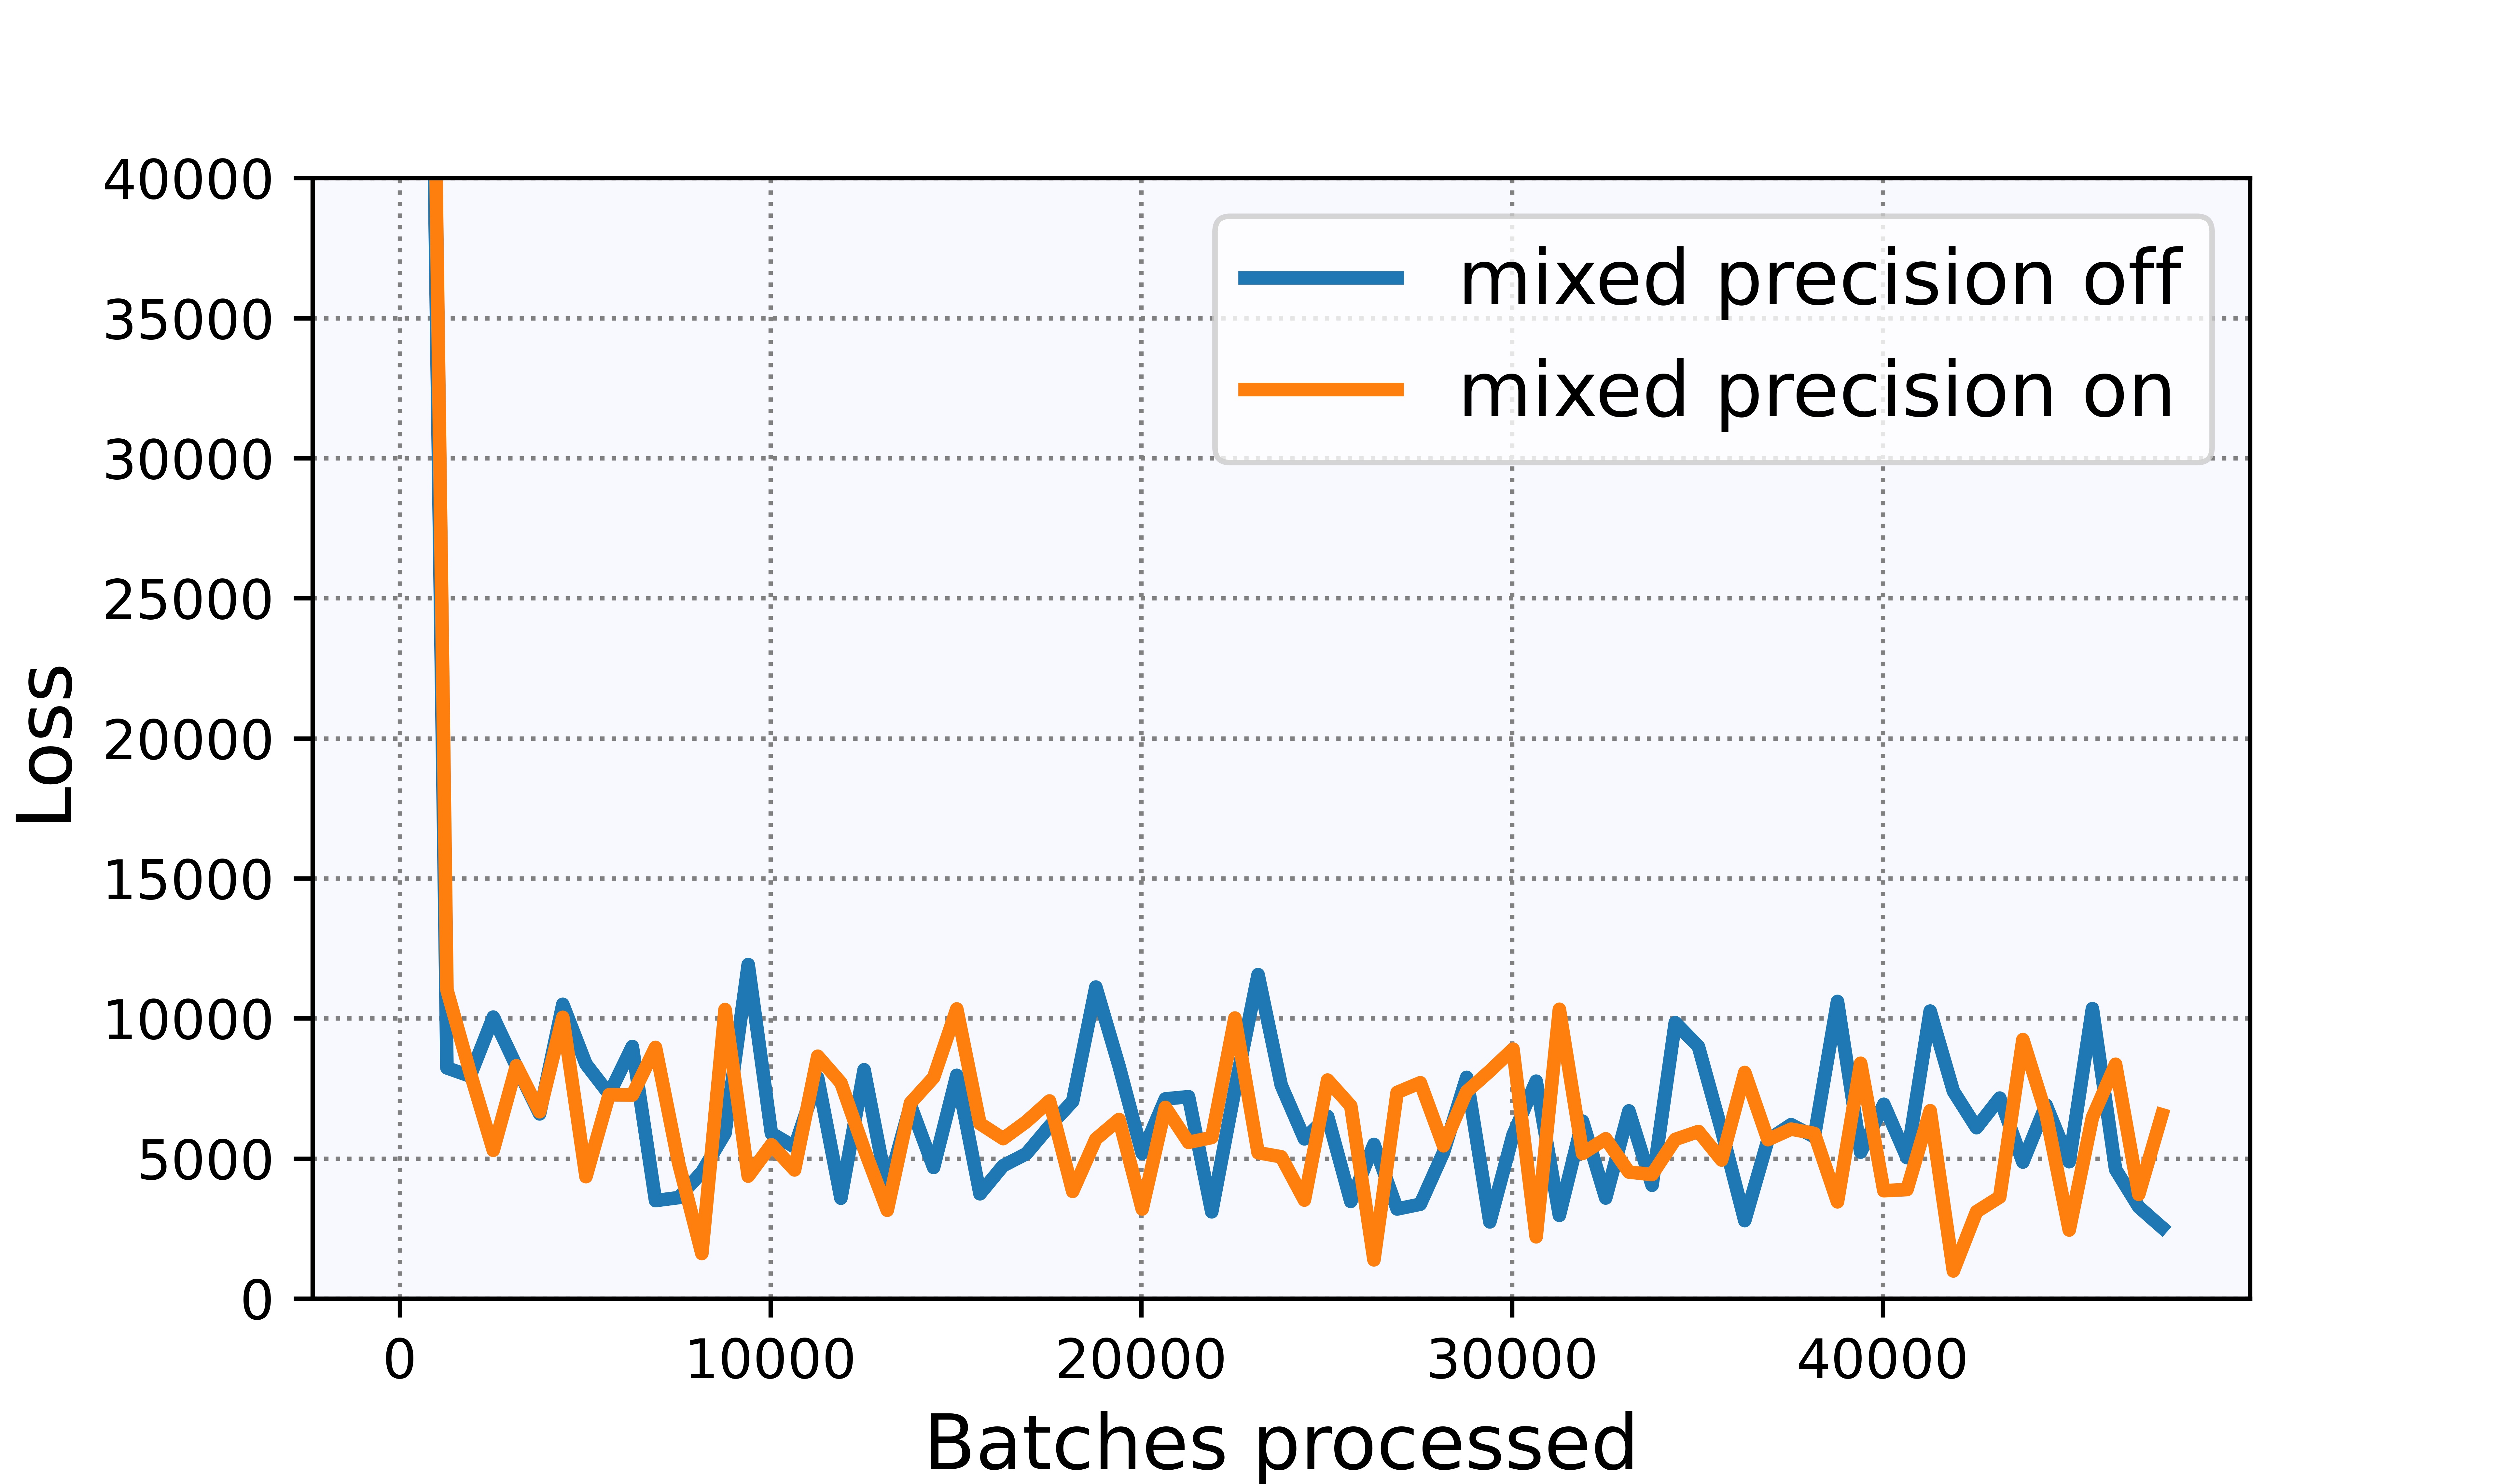
\includegraphics[width=\textwidth]{Chapters/figures/mixed_prec_rtx2080_loss.jpg}
         \caption{Loss curve RTX 2080 Ti}
    \end{subfigure}
    \begin{subfigure}[b]{0.49\textwidth}
        \centering
         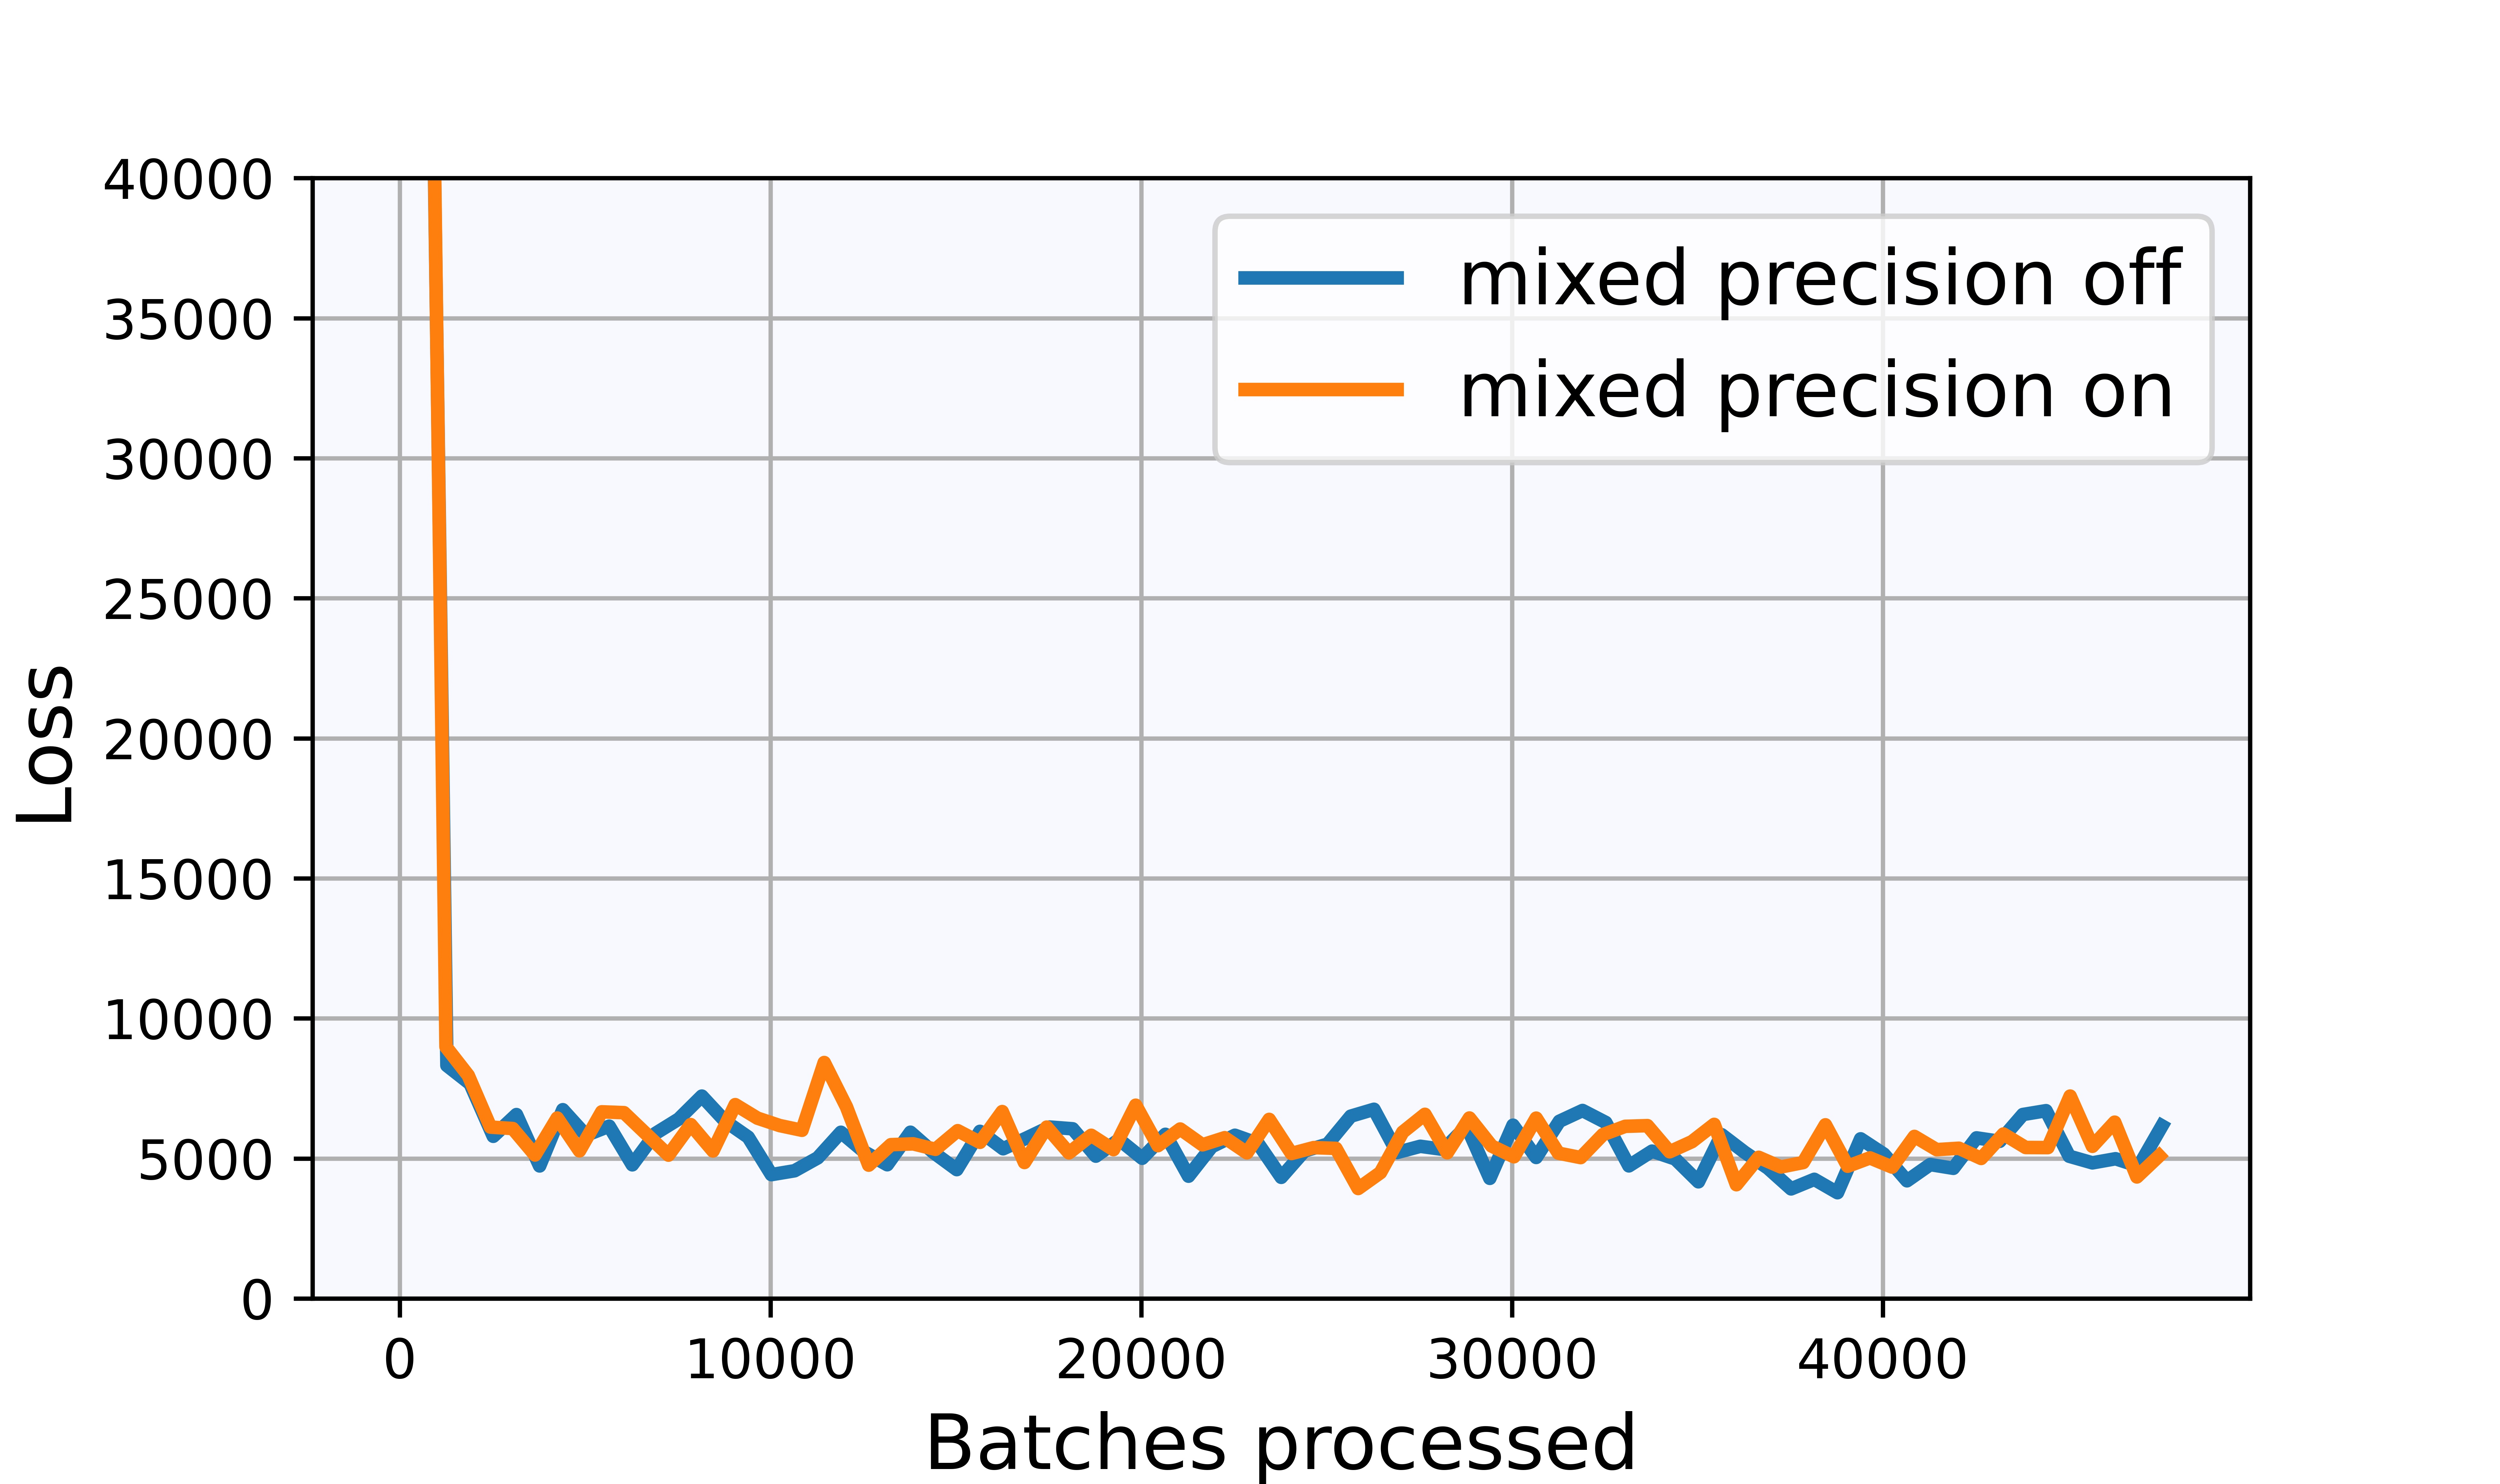
\includegraphics[width=\textwidth]{Chapters/figures/mixed_prec_a100_loss.jpg}
         \caption{Loss curve A100}
    \end{subfigure}
    \caption{Comparing loss curves for mixed precision \textbf{on} an \textbf{off} for both GPUs}
\end{figure}
%
\subsection{Training on arbitrary image sizes} %0.5-1
When training a generative model the image size the model gets as input for learning can have a large effect on what the model learns. Here not the total image size of the images is meant but the image size the model gets as input. As an example the cityscapes dataset (downscaled) consists of $256\times512$ pixel images. To reduce vRAM during training, the images from the dataset often are randomly cropped to another resolution, here $256\times256$. For some datasets this has only little negative effects on the model accuracy, e.g. for landscapes where the relative position of objects to each other only plays a minor role. But for datasets as the cityscapes dataset it is quite important for realistic results that the models learns the logic of images showing street scenes, i.e. learning that the street is in the middle, that there are parking cars on the left and right side of the image and so on. Training on too small crops can hinder the model to learn such logic.

As the version of NCSN \cite{score_3} does not support training on/sampling of non-square images, the model was adapted to do so. Actually the model already was able to process non-square images natively but there was a small bug that we fixed to make non-square training/sampling possible. To show the importance of this bugfix we investigate the influence of the above described effect on NCSN. For this purpose we trained two identical NCSN, one on $256\times256$ crops and one on the $256\times512$ original images. Some example results can be seen in \hyperref[tab:5.3]{Tab.\,5.3}. It is clearly visible that the full image model outperforms the cropped image model when the focus of evaluation is on street scene logic. It must be mentioned that for semantic image synthesis – the task for our experiments – this logic information actually is given by the semantic map which initially gives rise to the idea of training on crops at all. Nevertheless we suspect that a model knowing the logic without a semantic map also performs somewhat better than if it did not. For that reason models for further experiments on the cityscapes dataset were always trained with the full size images.
\begin{table}[] \label{tab:5.3}
    \centering
    \setlength\tabcolsep{-2pt}
    \begin{tabular}{ccc}
        & Training size $256\times256$ & \\
        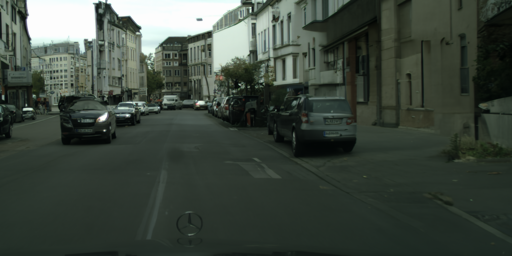
\includegraphics[width=0.33\textwidth]{Chapters/figures/experiments/crop/1_sample.png} &
        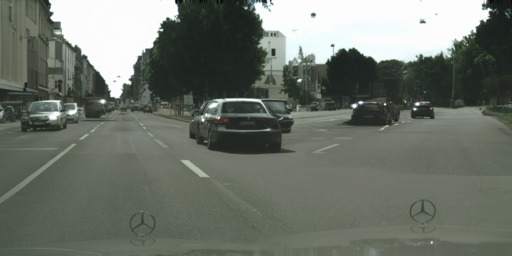
\includegraphics[width=0.33\textwidth]{Chapters/figures/experiments/crop/5_sample.png} &
        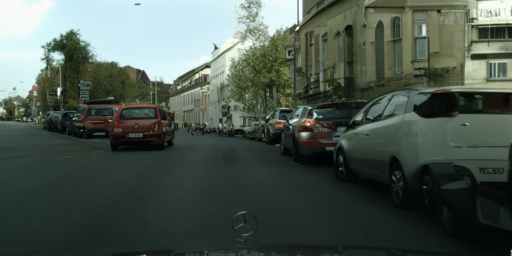
\includegraphics[width=0.33\textwidth]{Chapters/figures/experiments/crop/8_sample.png}\\
        & Training size $512\times256$ & \\ 
        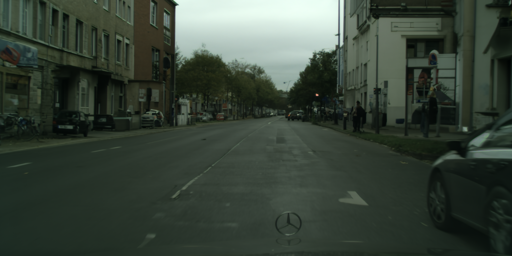
\includegraphics[width=0.33\textwidth]{Chapters/figures/experiments/crop/0_uncond_sample.png} &
        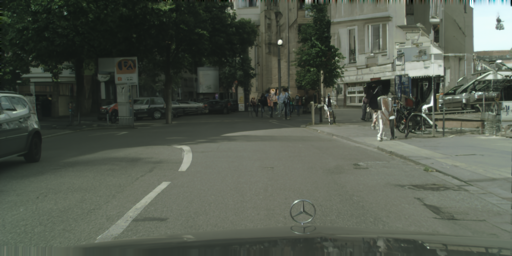
\includegraphics[width=0.33\textwidth]{Chapters/figures/experiments/crop/3_uncond_sample.png} &
        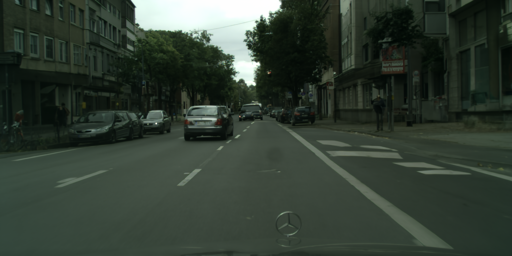
\includegraphics[width=0.33\textwidth]{Chapters/figures/experiments/crop/7_uncond_sample.png}
    \end{tabular}
    \caption{Unconditional example images of NCSN trained on cropped images (\textit{top}) and full size images (\textit{bottom}).}
    \label{tab:my_label}
\end{table}

%%%%%%%%%%%%%%%%%%%%%%%%%%%%%%%%%%%%%%%%%%%%%%%%%%%%%%%%%%%%%%%%%%%%%%%%%%%%%%%%%%%%%%%%%%%%%%%%%

\section{A competitive experiment on the Cityscapes dataset} %5-7
\section{Synthesizing high resolution landscapes} %5-7


\begin{figure}
    \tiny
    \centering
    \setlength\tabcolsep{-2pt}
    \begin{tabular}{cccc}
        Semantic map & Original image & T=0.8 & T=0.7 \\
        \includegraphics[width=0.25\textwidth]{Chapters/figures/experiments/seg_stop/0_1.0_seg_mask.png} &  \includegraphics[width=0.25\textwidth]{Chapters/figures/experiments/seg_stop/0_1.0_original.png} & 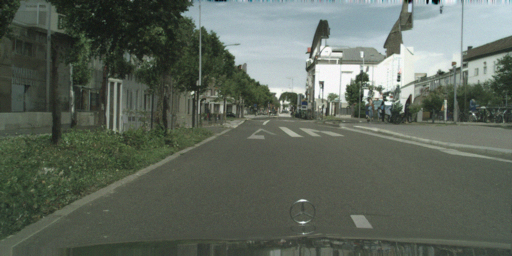
\includegraphics[width=0.25\textwidth]{Chapters/figures/experiments/seg_stop/0_0.8_cond_sample.png} & 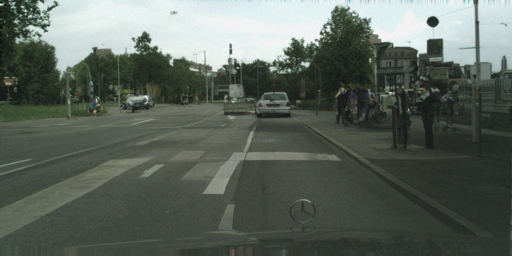
\includegraphics[width=0.25\textwidth]{Chapters/figures/experiments/seg_stop/0_0.7_cond_sample.png} \\
        T=0.65 & T=0.6 & T=0.55 & T=0.5\\
        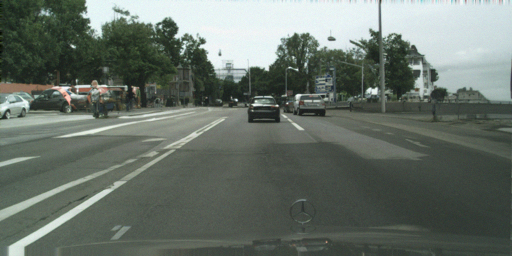
\includegraphics[width=0.25\textwidth]{Chapters/figures/experiments/seg_stop/0_0.6499999999999999_cond_sample.png} & 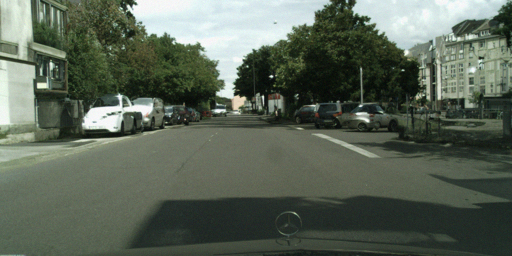
\includegraphics[width=0.25\textwidth]{Chapters/figures/experiments/seg_stop/0_0.6_cond_sample.png} & 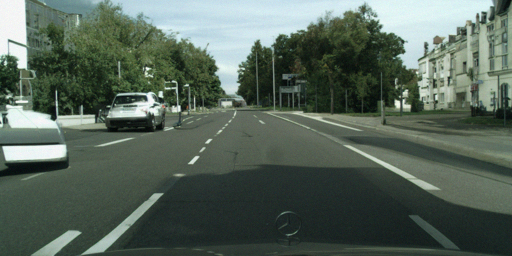
\includegraphics[width=0.25\textwidth]{Chapters/figures/experiments/seg_stop/0_0.55_cond_sample.png} & 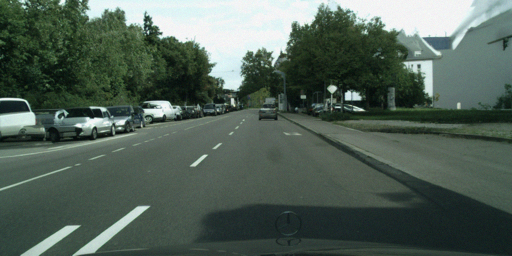
\includegraphics[width=0.25\textwidth]{Chapters/figures/experiments/seg_stop/0_0.5_cond_sample.png}\\
        T=0.45 & T=0.4 & T=0.2 & T=0\\
         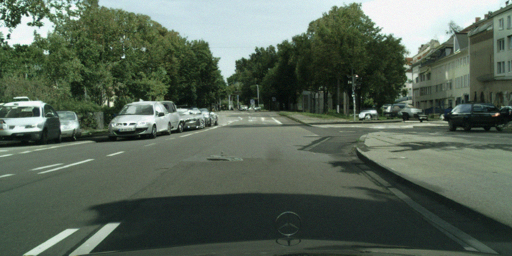
\includegraphics[width=0.25\textwidth]{Chapters/figures/experiments/seg_stop/0_0.44999999999999996_cond_sample.png} & 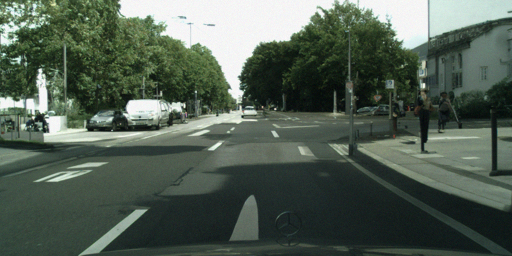
\includegraphics[width=0.25\textwidth]{Chapters/figures/experiments/seg_stop/0_0.3999999999999999_cond_sample.png} & 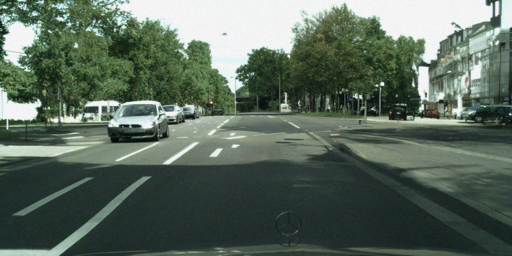
\includegraphics[width=0.25\textwidth]{Chapters/figures/experiments/seg_stop/0_0.19999999999999996_cond_sample.png}& 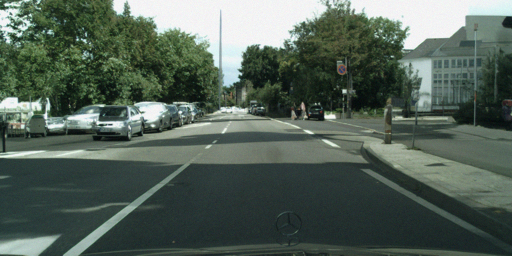
\includegraphics[width=0.25\textwidth]{Chapters/figures/experiments/seg_stop/0_0.0_cond_sample.png} 
    \end{tabular}
    \caption{Stop}
\end{figure}

\begin{figure}
    \tiny
    \centering
    \setlength\tabcolsep{-2pt}
    \begin{tabular}{cccc}
        Semantic map & Original image & T=0.2 & T=0.4  \\
        \includegraphics[width=0.25\textwidth]{Chapters/figures/experiments/seg_start/0_1.0_seg_mask.png} & 
        \includegraphics[width=0.25\textwidth]{Chapters/figures/experiments/seg_start/0_1.0_original.png} & 
        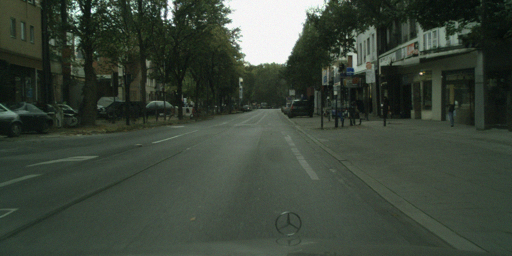
\includegraphics[width=0.25\textwidth]{Chapters/figures/experiments/seg_start/0_0.19999999999999996_cond_sample.png} & 
        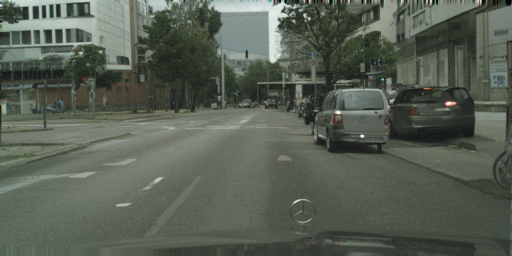
\includegraphics[width=0.25\textwidth]{Chapters/figures/experiments/seg_start/0_0.3999999999999999_cond_sample.png} \\
        T=0.5 & T=0.6 & T=0.65 & T=0.7  \\
        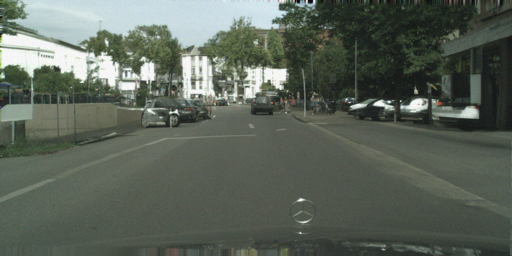
\includegraphics[width=0.25\textwidth]{Chapters/figures/experiments/seg_start/0_0.5_cond_sample.png} & 
        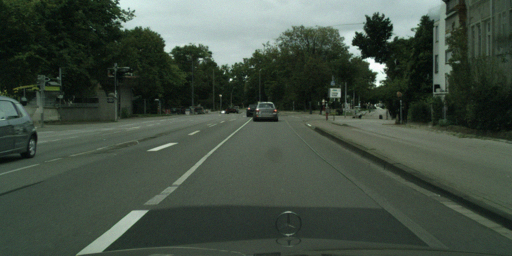
\includegraphics[width=0.25\textwidth]{Chapters/figures/experiments/seg_start/0_0.6_cond_sample.png} & 
        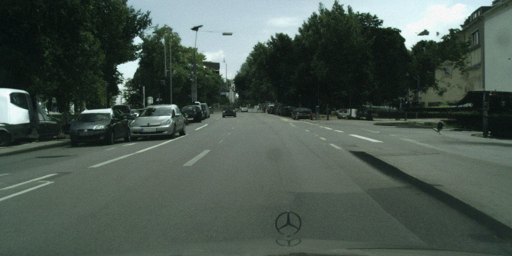
\includegraphics[width=0.25\textwidth]{Chapters/figures/experiments/seg_start/0_0.6499999999999999_cond_sample.png} &
        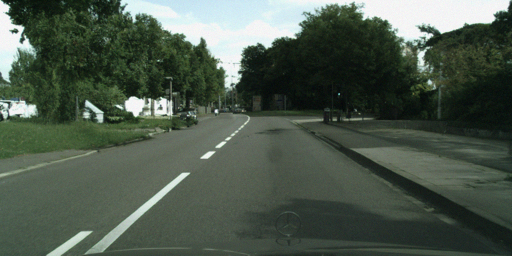
\includegraphics[width=0.25\textwidth]{Chapters/figures/experiments/seg_start/0_0.7_cond_sample.png}  \\
        T=0.75 & T=0.8 & T=0.9 & T=1  \\
        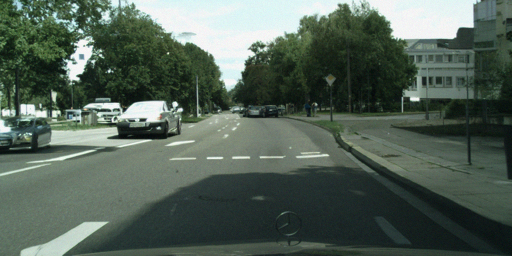
\includegraphics[width=0.25\textwidth]{Chapters/figures/experiments/seg_start/0_0.75_cond_sample.png} & 
        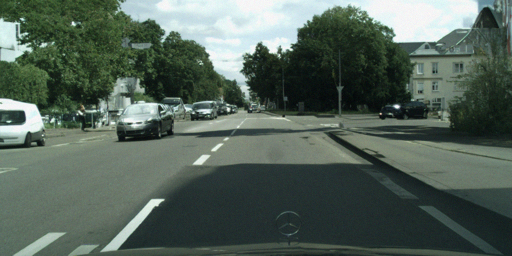
\includegraphics[width=0.25\textwidth]{Chapters/figures/experiments/seg_start/0_0.8_cond_sample.png} & 
        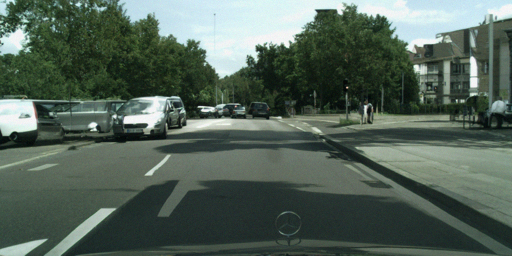
\includegraphics[width=0.25\textwidth]{Chapters/figures/experiments/seg_start/0_0.9_cond_sample.png} & 
        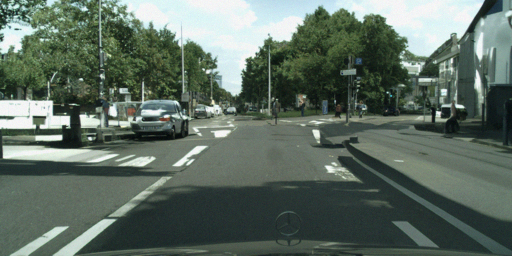
\includegraphics[width=0.25\textwidth]{Chapters/figures/experiments/seg_start/0_1.0_cond_sample.png}
    \end{tabular}
    \caption{Start}
    \label{tab:my_label}
\end{figure}